
\documentclass[12pt,a4paper]{article}
\usepackage[utf8]{inputenc}
\usepackage[russian]{babel}
\usepackage{amsmath}
\usepackage{amsfonts}
\usepackage{amssymb}
\usepackage{graphicx}
\usepackage{float}
\usepackage{listings}
\usepackage[left=2cm,right=2cm,top=2cm,bottom=2cm]{geometry}
\usepackage{tocloft}
\usepackage{placeins}

\usepackage{titlesec}
\usepackage{hyperref}

% section and subsection formmatting
\titleformat{\section}[block]{\normalfont\Large\bfseries\filcenter}{\thesection}{1em}{}
\titleformat{\subsection}{\normalfont\large\bfseries}{\thesubsection}{1em}{}

% Customize the table of contents to GOST standards
\renewcommand{\cftsecdotsep}{\cftdotsep}
\renewcommand{\cftsecfont}{\normalfont}
\renewcommand{\cftsecpagefont}{\normalfont}
\renewcommand{\cftsecpresnum}{\S\ }
\newlength{\stdindent}
\setlength{\stdindent}{\cftsecnumwidth}
\addtolength{\cftsecnumwidth}{3mm}

\numberwithin{subsection}{section}
\usepackage{xcolor}
\lstset{
basicstyle=\ttfamily,
columns=fullflexible,
frame=single,
breaklines=true,
postbreak=\mbox{\textcolor{red}{$\hookrightarrow$}\space},
keywordstyle=\color{blue},
commentstyle=\color{green},
}


\begin{document}

\begin{titlepage}
    \begin{center}
        \vspace*{2cm}
        {\Large \textbf{МИНИСТЕРСТВО НАУКИ И ВЫСШЕГО ОБРАЗОВАНИЯ РОССИЙСКОЙ ФЕДЕРАЦИИ}}\\
        \vspace{0.5cm}
        {\Large \textbf{ФЕДЕРАЛЬНОЕ ГОСУДАРСТВЕННОЕ АВТОНОМНОЕ ОБРАЗОВАТЕЛЬНОЕ УЧРЕЖДЕНИЕ ВЫСШЕГО ОБРАЗОВАНИЯ}}\\
        \vspace{0.5cm}
        {\Large \textbf{НОВОСИБИРСКИЙ НАЦИОНАЛЬНЫЙ ИССЛЕДОВАТЕЛЬСКИЙ ГОСУДАРСТВЕННЫЙ УНИВЕРСИТЕТ}}\\
        \vspace{0.5cm}
        {\large \textbf{Факультет информационных технологий}}\\
        \vspace{0.5cm}
        {\large \textbf{Кафедра параллельных вычислений}}\\
        \vspace{1cm}
         {\Large \textbf{ОТЧЕТ О ВЫПОЛНЕНИИ ПРАКТИЧЕСКОЙ РАБОТЫ}}
        \vspace{0.5cm}
        
        {\Large \textbf{Практическая работа №2}}\\
        \vspace{0.5cm}
         {\large Изучение оптимизирующего компилятора}\\
        \vspace{0.5cm}
        {\large студента 2 курса, группы 23201}\\
        \vspace{0.5cm}
        {\Large \textbf{Сорокина Матвея Павловича}}\\
        \vspace{1cm}
        {\large Направление 09.03.01 -- ''Информатика и вычислительная техника''}\\
        \vspace{2cm}
        
        \begin{flushright}
            \textbf{Преподаватель: А.С. Матвеев} \\
        \end{flushright}
        
        \vfill
        
        {\large Новосибирск, 2024 г.}
    \end{center}
\end{titlepage}

\tableofcontents

\newpage

\setcounter{page}{2}


\section{ЦЕЛЬ}
\begin{enumerate}
    \item Изучение основных функций оптимизирующего компилятора, некоторых примеров
     оптимизирующих преобразований и уровней оптимизации.
    \item Получение базовых навыков работы с компилятором \textit{GCC}.
    \item Анализ влияния различных уровней оптимизации компилятора \textit{GCC}
     на время выполнения программы.
\end{enumerate}


\section{ЗАДАНИЕ}
В ходе работы было необходимо выполнить следующие задачи:
\begin{enumerate}
    \item Написать программу на языке \textit{C} или \textit{C++}, которая реализует выбранный алгоритм из задания. 
    \item Проверить правильность работы программы на нескольких тестовых наборах входных данных. 
    \item Выбрать значение параметра N таким, чтобы время работы программы было порядка 30-60 секунд. 
    \item Программу скомпилировать компилятором GCC с уровнями оптимизации: \\
    -O0, -O1, -O2, -O3, -Os, -Ofast, -Og под архитектуру процессора \textit{x86}.
    \item Для каждого из семи вариантов компиляции измерить время работы программы при нескольких
    значениях \textit{N}. 
    \item Составить отчет по лабораторной работе.
\end{enumerate}

\newpage


\section{ОПИСАНИЕ РАБОТЫ}

%\setcounter{subsection}{0}
%\renewcommand{\thesubsection}{1.\arabic{subsection}}
% \subsection{}
\begin{enumerate}
    \item Реализовано задание №5 - алгоритм вычисления функции $e^x$ с помощью разложения 
    в ряд Маклорена по первым \textit{N} членам данного ряда на языке програмирования \textit{C++}.
    \\
    \\
    Для измерения времени работы программы использовалась библиотечная 
    функция \textit{clock\_gettime} из библиотеки \textit{time.h}.
    \\
    \\
    Время замерялось перед началом и после окончания работы функции, вычисляющей
    экспоненту в заданной степени. Разность этих двух значений дает общее время выполнения функции. 
    Для проверки точности измерений, код программы запускается несколько раз.

    \item Код программы также предоставлен (см. \hyperref[app:listing]{Приложение 1}), 
    также предоставлен \textit{bash-скрипт}, компилирующий и запускающий программу 
    с конкретными знаениями x и N, записывающий время вычисления экспоненциальной функции с 
    различными уровнями оптимизации компилятора \textit{GCC} в \textit{report.csv} 
    файл (см. \hyperref[app:listing]{Приложение 2}), после чего запускает
    \textit{create\_table.sh}, визуализирующий информацию из 
    \textit{report.csv} (см. \hyperref[app:listing]{Приложение 3}).

\end{enumerate}


\section{ЗАКЛЮЧЕНИЕ}
В ходе данной лабораторной работы мы познакомились с различными методами измерения 
работы программ и научились пользоваться ими на практике.
\\
\\
Также было установлено, что уровни оптимизации компилятора GCC оказывают влияние
на время выполнения программы. Было замечено, что с увеличением уровня оптимизации
время выполнения программы уменьшается.
\\
\\
Стоит обратить внимание на то, что наиболее распространенным ключом оптимизации 
является \textit{-O2}, поскольку:

\begin{enumerate}
    \item Ключ активирует большинство оптимизаций, которые улучшают 
    производительность и уменьшают размер кода, не добавляя экстремальных
     и потенциально нестабильных оптимизаций.
    \item Он улучшает скорость выполнения программы, при этом сохраняя её стабильность.
\end{enumerate}
\newpage


\section{ПРИЛОЖЕНИЯ}\label{app:listing}
%\addcontentsline{toc}{section}{Приложение}
%\setcounter{subsection}{0}
%\renewcommand{\thesubsection}{2.\arabic{subsection}}

\subsection*{Приложение 1: Исходный код программы \textit{ExponentCalculation.cpp}}
\begin{lstlisting}
    #include <iostream>
    #include <time.h>
    #include <cstdlib> // for atoi and atof
    #include <cmath> // for pow
    
    long double ExpCalculation(long double x, long long n) {
        long double exp = 1.0;
        long double term = 1.0;
    
        for (long long i = 1; i < n; i++) {
            term *= x / i;
            exp += term;
        }
    
        return exp;
    }
    
    int main(int argc, char *argv[]) {
        if (argc != 3) {
            std::cerr << "Usage: <degree> <number of terms>" << std::endl;
            return 0;
        }
    
        struct timespec start, end;
        long double x = atoll(argv[1]);
        long long n = atoll(argv[2]);
    
        std::cout << "x = " << x << ", n = " << n << std::endl;
    
        int runs = 3;
        double time_total = 0;
    
        for (long long i = 0; i < runs; i++) {
            clock_gettime(CLOCK_MONOTONIC_RAW, &start);
            long double exp = ExpCalculation(x, n);
            clock_gettime(CLOCK_MONOTONIC_RAW, &end);
    
            double taken_time = (end.tv_sec - start.tv_sec) + (end.tv_nsec - start.tv_nsec) / 1e9;
            std::cout << "e^(" << x << ") = " << exp << std::endl;
            std::cout << "Run " << i + 1 << " took " << taken_time << " seconds to complete" << "\n" << std::endl;
            time_total += taken_time;
        }
    
        std::cout << "Average time: " << time_total / runs << " seconds" << std::endl;
        return 0;
    }
        
\end{lstlisting}

\subsection*{Приложение 2: bash-скрипт \textit{compile\_and\_run.sh}, для компиляции и запуска программы 
\textit{SinCalculation.cpp}, записи результата в файл report.csv}

\begin{lstlisting}
    #!/bin/bash

    input="ExponentCalculation.cpp"

    optimization_keys=("-O0" "-O1" "-O2" "-O3" "-Os" "-Ofast" "-Og")
    n=("4000000000" "4500000000" "5000000000")
    x=90

    echo "Optimixation level, N value, Time taken (seconds)" > report.csv

    for i in "${optimization_keys[@]}"; do
        for j in "${n[@]}"; do
            g++ $input $i -std=c++11
            output=$(./a.out $x $j | grep "Average time:" | awk '{print $3}')
            echo "$i, $j, $output" >> report.csv
        done
    done

    echo "Successfully generated report.csv"
\end{lstlisting}


\subsection*{Приложение 3: \textit{bash-скрипт} \textit{create\_table.sh} для вывода в 
табличном формате данных из файла \textit{report.csv}}

\begin{verbatim}
    #!/bin/bash

    if [ ! -f report.csv ]; then
        echo "report.csv not found!"
        exit 1
    fi

    # Вывод заголовка таблицы
    echo -e "Оптимизация\t N\t\t Время выполнения (сек)"

    # -F',': запятая в качестве разделителя столбцов
    # NR>1: пропускаем первую строку
    awk -F',' 'NR>1 { printf "%s\t\t%s\t%s\t%s\n", $1, $2, $3, $4 }' report.csv

\end{verbatim}

\newpage


\subsection*{Приложение 4: Результаты измерений}

\begin{table}[H]
\centering
\begin{tabular}{|c|c|c|}
\hline
Оптимизация & Значение \(N\) & Время выполнения (с) \\
\hline
-O0 & 4,000,000,000 & 35.1887 \\
-O0 & 4,500,000,000 & 39.8341 \\
-O0 & 5,000,000,000 & 43.9038 \\
\hline
-O1 & 4,000,000,000 & 8.04768 \\
-O1 & 4,500,000,000 & 9.01514 \\
-O1 & 5,000,000,000 & 9.90664 \\
\hline
-O2 & 4,000,000,000 & 7.84239 \\
-O2 & 4,500,000,000 & 8.87028 \\
-O2 & 5,000,000,000 & 9.99184 \\
\hline
-O3 & 4,000,000,000 & 7.96013 \\
-O3 & 4,500,000,000 & 8.82066 \\
-O3 & 5,000,000,000 & 9.77772 \\
\hline
-Os & 4,000,000,000 & 8.39481 \\
-Os & 4,500,000,000 & 9.47931 \\
-Os & 5,000,000,000 & 10.3841 \\
\hline
-Ofast & 4,000,000,000 & 7.8265 \\
-Ofast & 4,500,000,000 & 8.91898 \\
-Ofast & 5,000,000,000 & 10.0095 \\
\hline
-Og & 4,000,000,000 & 7.99961 \\
-Og & 4,500,000,000 & 8.88734 \\
-Og & 5,000,000,000 & 9.85844 \\
\hline
\end{tabular}

\caption{Результаты измерения времени выполнения программы}
\label{tab:measurements}

\end{table}


\subsection*{Приложение 5: График зависимости времени от оптимизации компиляции
 и параметра N для разных уровней оптимизации}

\begin{figure}[H]
    \centering
    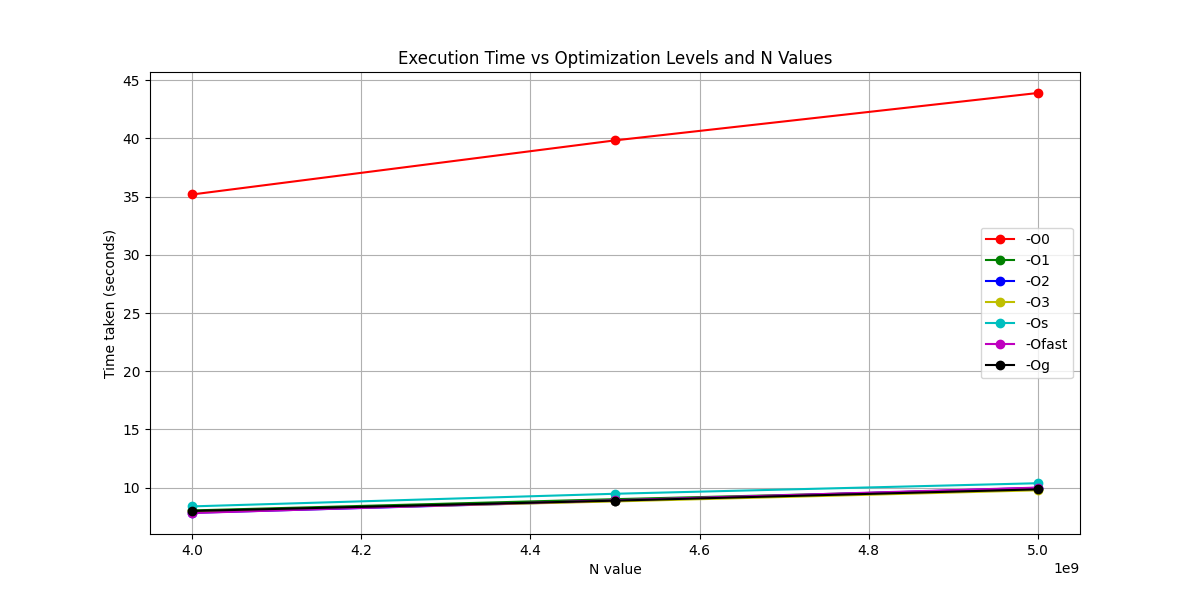
\includegraphics[width=0.8\textwidth]{5.png}
    \caption{График зависимости времени от N}
\end{figure}

\newpage


\subsection*{Приложение 6: Скрипт для визуализации графика зависимости времени
 от зависимости компиляции на языке \textit{Python}}

\begin{lstlisting}
import matplotlib.pyplot as plt

n_values = [4000000000, 4500000000, 5000000000]

times_o0 = [35.1887, 39.8341, 43.9038]
times_o1 = [8.04768, 9.01514, 9.90664]
times_o2 = [7.84239, 8.87028, 9.99184]
times_o3 = [7.96013, 8.82066, 9.77772]
times_os = [8.39481, 9.47931, 10.3841]
times_ofast = [7.8265, 8.91898, 10.0095]
times_og = [7.99961, 8.88734, 9.85844]

plt.figure(figsize=(12, 6))

plt.plot(n_values, times_o0, 'r-o', label='-O0')
plt.plot(n_values, times_o1, 'g-o', label='-O1')
plt.plot(n_values, times_o2, 'b-o', label='-O2')
plt.plot(n_values, times_o3, 'y-o', label='-O3')
plt.plot(n_values, times_os, 'c-o', label='-Os')
plt.plot(n_values, times_ofast, 'm-o', label='-Ofast')
plt.plot(n_values, times_og, 'k-o', label='-Og')

plt.xlabel('N value')
plt.ylabel('Time taken (seconds)')
plt.legend()
plt.grid(True)


plt.show()
\end{lstlisting}

\end{document}
